\documentclass{BHCexam}	
\usepackage{yhmath}%弧度表示
\newcommand{\xl}[2]{\vv{#1}\bm\cdot\vv{#2}}
\begin{document}
\biaoti{平面向量}
\fubiaoti{}
\maketitle
\begin{questions}

\qs
已知向量$ \vv{a}=(1,m),~\vv{b}=(3,-2) $,且$\left(\vv{a}+\vv{b}\right)\bot \vv{b} $,则$m$=\xx
\onech{$-8$}{$-6$}{$6$}{$8$}
\qs 若向量$ \bm{a,b,c} $满足$ \bm{a}\sslash\bm{b} $且$ \bm{a}\bot\bm{c} $,则$ \bm{c\cdot\left(a+2b\right)} =$\xx
\onech{$ 4$}{$ 3$}{$ 2$}{$ 0$}

\qs 若向量$ \bm{a,b} $满足:$ \abs{\bm{a}}=1,~\bm{\left(a+b\right)}\bot \bm{a},~\bm{\left(2a+b\right)}\bot \bm{b} $,~则$ \abs{\bm{b}}= $\xx
\onech{$ 2$}{$ \sqrt{2}$}{$ 1$}{$ \dfrac{\sqrt{2}}{2}$}
\qs 已知两个非零向量$\bm{ a,b}$满足$ \abs{\bm{a+b}}=\abs{\bm{a-b}} $,则下面结论正确的是\xx
\twoch{$ \bm{a}\sslash \bm{b}$}{$ \bm{a}\bot\bm{b}$}{$\abs{\bm{a}}=\abs{\bm{b}} $}{$ \bm{a}+\bm{b}=\bm{a}-\bm{b}$}
\qs 若向量$ \bm{a} $与$ \bm{b} $不共线,$ \bm{a}\cdot \bm{b}\ne 0,~ $且$\bm{c}=\bm{a}-\left(\dfrac{\bm{a\cdot a}}{\bm{a\cdot b}}\right)\bm{\cdot b} $,则向量$ \bm{a} $与$ \bm{c} $的夹角为\xx
\onech{$ 0$}{$ \dfrac{\pi}{6}$}{$ \dfrac{\pi}{3}$}{$ \dfrac{\pi}{2}$}
\qs
设向量$\vv{a}$,$\vv{b}$满足$\left|\vv{a}+\vv{b}\right|=\sqrt{10}$,$\left|\vv{a}-\vv{b}\right|=\sqrt{6}$,则$\xl{a}{b}=$\xx
\onech{$1$}{$2$}{$3$}{$5$}


\qs 已知$ O,~A,~B $是平面上的三个点,直线$ AB $上有一点$ C $,满足$ 2\vv{AC}+\vv{CB}=\mathbf{0}, ~$则$ \vv{OC}= $\xx
\twoch{$ 2\vv{OA}-\vv{OB} $}{$ -\vv{OA}+2\vv{OB} $}{$\dfrac{2}{3}\vv{OA}-\dfrac{1}{3}\vv{OB}$}{$ -\dfrac{1}{3}\vv{OA}+\dfrac{2}{3}\vv{OB} $}
\qs 设$ D $为$\triangle ABC$所在平面内一点,$ \vv{BC}=3\vv{CD} $,则\xx
\twoch{$ \vv{AD}=-\dfrac{1}{3}\vv{AB}+\dfrac{4}{3}\vv{AC}$}{$ \vv{AD}=\dfrac{1}{3}\vv{AB}-\dfrac{4}{3}\vv{AC}$}{$ \vv{AD}=\dfrac{4}{3}\vv{AB}+\dfrac{1}{3}\vv{AC}$}{$ \vv{AD}=\dfrac{4}{3}\vv{AB}-\dfrac{1}{3}\vv{AC}$}
\qs 平面上$ O,A,B $三点不共线,设$ \vv{OA}=\bm{a},~\vv{OB}=\bm{b},~ $则$ \triangle OAB $的面积等于\xx
\twoch{$ \sqrt{\abs{\bm{a}}^2\abs{\bm{b}}^2-\left(\bm{a\cdot b}\right)^2}$}{$ \sqrt{\abs{\bm{a}}^2\abs{\bm{b}}^2+\left(\bm{a\cdot b}\right)^2}$}{$ \dfrac{1}{2}\sqrt{\abs{\bm{a}}^2\abs{\bm{b}}^2-\left(\bm{a\cdot b}\right)^2}$}{$\dfrac{1}{2}\sqrt{\abs{\bm{a}}^2\abs{\bm{b}}^2+\left(\bm{a\cdot b}\right)^2} $}
\qs 已知$ \bm{a}=(\sqrt{3},1) $,若将向量$ -2\bm{a} $绕坐标原点逆时针旋转$ 120^{\circ} $得到向量$ \bm{b} $,则$ \bm{b} $的坐标为\xx
\twoch{$ (0,4)$}{$ \left(2\sqrt{3},-2\right)$}{$ \left(-2\sqrt{3},2\right)$}{$ \left(2,-2\sqrt{3}\right)$}

\qs 设$ \bm{m},\bm{n} $是非零向量,则“存在负数$ \lambda $,使得$ \bm{m}=\lambda\bm{n} $”是“$ \bm{m\cdot n}<0 $”的\xx
\twoch{充分而不必要条件}{必要而不充分条件}{充分必要条件}{既不充分也不必要条件}
\qs 设$ \vv{a},\vv{b} $是向量,则“$ \left|\vv{a}\right|=\left|\vv{b}\right| $”是“$ \left|\vv{a}+\vv{b}\right|=\left|\vv{a}-\vv{b}\right| $”的\xx
\twoch{充分而不必要条件}{必要而不充分条件}{充分必要条件}{既不充分也不必要条件}

\qs $\vv{a},\vv{b} $为非零向量,“$ \vv{a}\bot\vv{b} $”是“函数$ f(x)=(x\vv{a}+\vv{b})\bm\cdot(x\vv{b}-\vv{a}) $为一次函数”的\xx
\twoch{充分而不必要条件}{必要而不充分条件}{充分必要条件}{既不充分也不必要条件}
\qs 设$ \vv{a},\vv{b} $是非零向量,“$ \xl{a}{b}=\left|\vv{a}\right|\left|\vv{b}\right| $”是“$ \vv{a}\sslash\vv{b} $”的\xx
\twoch{充分而不必要条件}{必要而不充分条件}{充分必要条件}{既不充分也不必要条件}

\qs 设平面向量$ \vv{a},~\vv{b},~\vv{c} $均为非零向量,则“$ \vv{a}\bm\cdot\left(\vv{b}-\vv{c}\right)=0 $”是“$\vv{b}=\vv{c}$”的\xx
\twoch{充分而不必要条件}{必要而不充分条件}{充分必要条件}{既不充分也不必要条件}  
\qs 设$ E,~F $分别是正方形$ ABCD $的边$ AB,~BC $上的点,且$AE=\dfrac{1}{2}AB,~BF=\dfrac{2}{3}BC,~$如果$ \vv{EF}=m\vv{AB}+n\vv{AC}(m,n\text{为实数}) ,~$那么$ m+n $的值为\xx
\onech{$ -\dfrac{1}{2} $}{$0$}{$\dfrac{1}{2}$}{1}
\qs 已知三角形$\triangle ABC$是边长为$ 1 $的等边三角形,点$ D,~E $分别是边$ AB,BC $的中点,连接$ DE $并延长到点$ F $,使得$ DE=2EF $,则$ \xl{AF}{BC} $的值是\xx
\onech{$ -\dfrac{5}{8}$}{$ \dfrac{1}{8}$}{$ \dfrac{1}{4}$}{$ \dfrac{11}{8}$}
\qs 已知菱形$ ABCD $的边长为$ 2,~  \angle BAD=120^{\circ} $,点$ E,~F $分别在边$ BC,~DC $上,$ BE=\lambda BC,~DF=\mu DC $,若$ \xl{AE}{AF}=1,~\xl{CE}{CF}=-\dfrac{2}{3} $,则$ \lambda+\mu= $\xx
\onech{$ \dfrac{1}{2}$}{$ \dfrac{2}{3}$}{$ \dfrac{5}{6}$}{$ \dfrac{7}{12}$}
\qs 已知$\triangle ABC$和点$ M $满足$ \vv{MA}+\vv{MB}+\vv{MC}=\bm{0}. $若存在实数$ m $使得$ \vv{AB}+\vv{AC}=m\vv{AM} $成立,则$ m= $\xx
\onech{$ 2$}{$ 3$}{$ 4$}{$ 5$}
\qs 已知$ O $是$ \triangle ABC $所在平面内一点,$ D $为$ BC $边中点,且$ 2\vv{OA}+\vv{OB}+\vv{OC}=\bm{0}. $那么\xx
\onech{$ \vv{AO}=\vv{OD}$}{$ \vv{AO}=2\vv{OD}$}{$ \vv{AO}=3\vv{OD}$}{$2\vv{AO}=\vv{OD} $}
\qs 在平行四边形$ ABCD $中,$ AC $与$ BD $交于点$ O,~E $是线段$ OD $的中点,$ AE $的延长线与$ CD $交于点$ F $.若$ \vv{AC}=\bm{a},~\vv{BD}=\bm{b},~ $则$ \vv{AF}= $\xx
\twoch{$ \dfrac{1}{4}\bm{a}+\dfrac{1}{2}\bm{b}$}{$\dfrac{1}{3}\bm{a}+\dfrac{2}{3}\bm{b} $}{$\dfrac{1}{2}\bm{a}+\dfrac{1}{4}\bm{b} $}{$\dfrac{2}{3}\bm{a}+\dfrac{1}{3}\bm{b} $}
\qs 已知平面上三点$ A,~B,~C $满足$ \abs{\vv{AB}}=6,~\abs{\vv{AC}}=8,~\abs{\vv{BC}}=10,~ $则$ \vv{AB}\bm{\cdot}\vv{BC}+\vv{BC}\bm{\cdot}\vv{CA}+\vv{CA}\bm{\cdot}\vv{AB}= $\xx
\onech{$ 48$}{$ -48$}{$ 100$}{$ -100$}
\qs 已知$\bm{e}_1,\bm{e}_2$为平面上的单位向量,$\bm{e}_1$与$\bm{e}_2$的起点均为坐标原点$ O $,$\bm{e}_1$与$\bm{e}_2$的夹角为$ \dfrac{\pi}{3} $,平面区域$ D $由所有满足$ \vv{OP}=\lambda \bm{e}_1+\mu \bm{e}_2 $的点$ P $组成,其中$ \left\{\begin{aligned}
&\lambda+\mu\le1,\\
&\lambda\ge0,\\
&\mu\ge0.
\end{aligned}\right. $那么平面区域$ D $的面积为\xx
\onech{$ \dfrac{1}{2}$}{$ \sqrt{3}$}{$ \dfrac{\sqrt{3}}{2}$}{$ \dfrac{\sqrt{3}}{4}$}
\qs 如图,在等腰梯形$ ABCD $中,$ AB=8,~BC=4,~CD=4,~ $点$ P $在线段$ AD $上运动,则$\left|\vv{PA}+\vv{PB}\right| $的取值范围是\xx
\onech{$ \left[6,4+4\sqrt{3}\right] $}{$\left[4\sqrt{2},8\right] $}{$ \left[4\sqrt{3},8\right] $}{$ \left[6,12\right] $}
\vspace{-2em}
\begin{center}
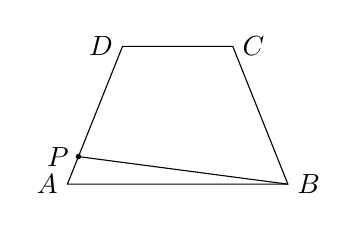
\begin{tikzpicture}[scale=0.7]
%\draw[help lines] (0,0) grid (4,4);
\draw (0,0) node[left](A){$A$} --(4,0)node[right](B){$B$} -- (3,2.5) node[right](C) {$C$}--(1,2.5) node[left](D){$D$}--cycle;
\coordinate[label=left:$P$] (P) at (0.2,0.5);
\draw[fill] (P) circle (1.1pt); 
\draw (P)--(4,0);
\end{tikzpicture}
\end{center}
\qs
已知向量$ \vv{a},\vv{b} $满足$ |\vv{a} |=1,\vv{b}=(2,1)$,且$ \lambda \vv{a}+\vv{b}=\bm{0}~(\lambda\in\mathbf{R}) $,则$ |\lambda |= $\tk.


\question
已知$A,B,C$是圆$O$上的三点,若$\vv{AO}=\dfrac{1}{2}\left(\vv{AB}+\vv{AC}\right)$,则$\vv{AB}$与$\vv{AC}$的夹角为\tk.
\qs 已知两个单位向量$\vv{a}$,$\vv{b}$的夹角为$60^{\circ}$,$\vv{c}=t\vv{a}+(1-t)\vv{b}$,若$\xl{b}{c}=0$,则$t=$\tk.
\qs 平面向量$\bm{a}=\left(1,2\right),\bm{b}=\left(4,2\right),\bm{c}=m\bm{a}+\bm{b}\left(m\inR\right) $且$\bm{c} $与$ \bm{a} $的夹角等于$ \bm{c} $与$ \bm{b} $的夹角,则$ m= $\tk.
\qs 已知点$ P $在圆$ x^2+y^2=1 $上,点$ A $的坐标为$ (-2,0) $,$ O $为原点,则$ \vv{AO}\bm{\cdot}\vv{AP} $的最大值为\tk.

\qs 已知单位向量$ \bm{e}_1\text{与}\bm{e}_2 $的夹角为$ \alpha $,且$ \cos \alpha =\dfrac{1}{3},~$向量$ \bm{a}=3\bm{e}_1-2\bm{e}_2 $与$ \bm{b}=3\bm{e}_1-\bm{e}_2 $的夹角为$ \beta $,则$ \cos \beta =$\tk.
\qs 在三角形$\triangle ABC$中,点$ M,N $满足$ \vv{AM}=2\vv{MC} ,~$$ \vv{BN}=\vv{NC} .~$若$ \vv{MN}=x\vv{AB}+y\vv{AC} $,则$ x= $\tk;$~ y= $\tk.
\qs 已知点$ A(1,-1) ,B(3,0),C(2,1).$若平面区域$ D $由所有满足$ \vv{AP}=\lambda \vv{AB}+\mu \vv{AC}~(1\le \lambda \le 2,0\le \mu \le 1) $的点$ P $组成,则$ D $的面积为\tk.

\qs 已知正方形$ ABCD $的边长为1,点$ E $是AB边上的动点,则$ \vv{DE}\cdot \vv{CB} $的值为\tk;~$ \vv{DE}\bm\cdot \vv{DC} $的最大值为\tk.

\qs 已知$ M $为$\triangle ABC$所在平面内的一点,且$ \vv{AM}=\dfrac{1}{4}\vv{AB}+n\vv{AC}. $若点$ M $在$\triangle ABC$内部(不含边界),则实数$ n $的取值范围是\tk. 
\qs 已知向量序列:$ \bm{a}_1,\bm{a}_2,\bm{a}_3,\cdots,\bm{a}_n,\cdots $满足如下条件:$ \left|\bm{a}_1\right|=4\left|\bm{d}\right|=2,~2\bm{a}_1\bm\cdot \bm{d}=-1 $且$ \bm{a}_n-\bm{a}_{n-1}=
\bm{d}~(n=,3,4,\cdots). $若$ \bm{a}_1\bm{\cdot}\bm{a}_k=0,~ $则$ k= $\tk;~$ \left|\bm{a}_1\right|,~  \left|\bm{a}_2\right|, \left|\bm{a}_3\right|,\cdots, \left|\bm{a}_n\right|,\cdots$中第\tk 项最小.
\qs 如图,$ \triangle AB_1C_1,~\triangle C_1B_2C_2,~\triangle C_2B_3C_3 $是三个边长为2的等边三角形,且有一条边在同一直线上,边$ B_3C_3 $上有两个不同的点$ P_1,~P_2,~ $则$ \vv{AB_2}\bm{\cdot}(\vv{AP_1}+\vv{AP_2}) =$\tk.
\begin{center}
\begin{tikzpicture}
%\draw[help lines](0,0) grid (6,2);
\tikzmath{
\a=sqrt(3);
}
\coordinate[label=below:$A$](A) at (0,0);
\foreach \p in {1,2,3}
\coordinate[label=below:$C_{\p}$] (C_\p) at($(\p*2,0)$) ;
\foreach \q in {1,2,3}
\coordinate[label=above:$B_{\q}$] (B_\q) at($(2*\q-1,\a)$);
\foreach \r in{1,2,3}
\draw (B_\r)--(C_\r);
\draw (A)--(C_3) (A)--(B_1) (C_1)--(B_2) (C_2)--(B_3);
\draw[->,>=stealth] (A)--(B_2) ;
\draw[->,>=stealth](A)--($(B_3)!0.3!(C_3)$) node[right](P_1){$P_1$};
\draw[->,>=stealth](A)--($(B_3)!0.7!(C_3)$) node[right](P_2){$P_2$};

\end{tikzpicture}
\end{center}

\qs 向量$ \vv{a},~\vv{b},\vv{c} $在正方形网格中的位置如图所示,若$ \vv{c}=\lambda\vv{a}+\mu\vv{b}~(\lambda,\mu \in \mathbf{R}) $,则$ \dfrac{\lambda}{\mu}=$\tk.
\begin{center}
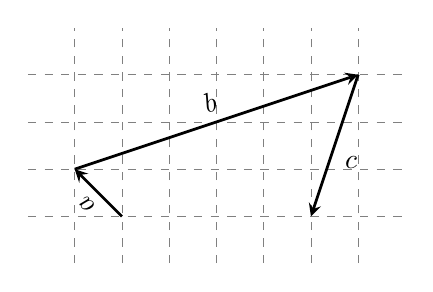
\begin{tikzpicture}[line width=1 pt,scale=0.6]
\draw[help lines,smooth, dashed] (-3.99,-2.99) grid (3.99,1.99);
\draw [->,>=stealth](-2,-2)--(-3,-1) node[sloped,midway,left,above,rotate=180](a){$\large\vv{a}$};
\draw [->,>=stealth](-3,-1)--(3,1) node[sloped,midway,left,above](b){$\large\vv{b}$};
\draw [->,>=stealth](3,1)--(2,-2) node[midway,below right ](c){$\large\vv{c}$};

\end{tikzpicture}
\end{center}
\qs 在$\triangle ABC$中,点$ M,N $满足$ \vv{AM}=2\vv{MC},~\vv{BN}=\vv{NC}. $若$ \vv{MN}=x\vv{AB}+y\vv{AC},~ $则$ x= $\tk;\\
$ y= $\tk.
\vspace{-2em}
\begin{center}
\begin{tikzpicture}
\draw(0,0)node[below](B){\small$B$}--(1,0)node[below](N){\small$N$}--(2,0)node[below](C){\small$C$};
\draw (0,0)--(1.1,2.1)node[above](A){\small$A$}--(2,0);
\draw (1,0)--(1.1,2.1);
\draw(1,0)--($(1.1,2.1)!0.7!(2,0)$)node[right](M){\small$M$};
\end{tikzpicture}
\end{center}

\qs 如图,在平行四边形$ ABCD $中,$ AP\bot BD~ $,垂足为$ P $,且$ AP=3 $,则$ \xl{AP}{AC}= $\tk.\begin{center}
\begin{tikzpicture}
%\draw[help lines](0,0) grid (4,4);
\coordinate [label=below:$B$](B) at(0,0);
\coordinate [label=below:$C$](C) at(3,0);
\coordinate [label=$A$](A) at(1,1.5);
\coordinate [label=$D$](D) at(4,1.5);
\draw (A)--(B)--(C)--(D)--cycle (A)--(C) (B)--(D);
\coordinate[label=below:$P$] (P) at($(B)!(A)!(D)$);
\draw (A)--(P);
\end{tikzpicture}
\end{center}
\vspace{-2em}
\qs 给定两个长度为$ 1 $的平面向量$ \vv{OA} $和$ \vv{OB} $,它们的夹角为$ 120^{\circ} $.如图所示,点$ C $在以$ O $为圆心的圆弧$ \wideparen{AB} $上变动,若$ \vv{OC}=x\vv{OA}+y\vv{OB} $,其中$ x,~y\inR $,则$ x+y $的最大值是\tk.
\begin{center}
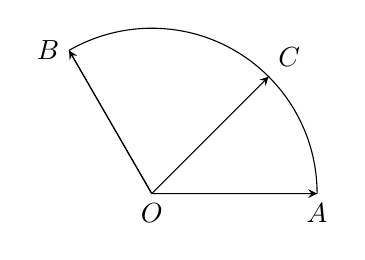
\begin{tikzpicture}[scale=0.7]
\coordinate[label=below:$O$](O) at(0,0);
\coordinate[label=below:$A$](A) at(0:3);
\coordinate[label=left:$B$](B) at(120:3);
\draw (O)--(A) (O)--(B);
\draw (3,0) arc (0:120:3);
\coordinate [label=above right:$C$](C) at(45:3);
\foreach \p in {A,B,C}
\draw[->,>=stealth](O)--(\p);
\end{tikzpicture}
\end{center}
\vspace{-2em}
\qs 如图,半径为$ \sqrt{3} $的扇形$ AOB $的圆心角为$ 120^{\circ} $,点$ C $在弧$ AB $上,且$ \angle COB=30^{\circ} $.若$ \vv{OC}=\lambda\vv{OA}+\mu\vv{OB} ,~$则$ \lambda+\mu= $\tk.
\begin{center}
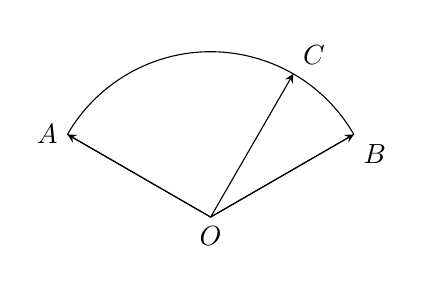
\begin{tikzpicture}[rotate=30,scale=0.7]
\coordinate[label=below:$O$](O) at(0,0);
\coordinate[label= below right:$B$](A) at(0:3);
\coordinate[label=left:$A$](B) at(120:3);
\draw (O)--(A) (O)--(B);
\draw (3,0) arc (0:120:3);
\coordinate [label=above right:$C$](C) at(30:3);
\foreach \p in {A,B,C}
\draw[->,>=stealth](O)--(\p);
\end{tikzpicture}
\end{center}
%\vspace{-2em}
\qs 在梯形$ ABCD $中,$ AB\sslash DC ,~AD\bot AB,AD=DC=\dfrac{1}{2}AB=2.$点$ N $是$ CD $边上的一动点,则$ \vv{AN}\bm{\cdot}\vv{AB} $的最大值为\tk.
\begin{center}
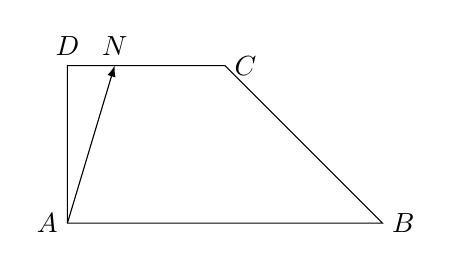
\begin{tikzpicture}
\coordinate[label=left:$A$] (A) at(0,0);
\coordinate[label=right:$B$] (B) at(4,0);
\coordinate[label=above:$D$] (D) at(0,2);
\coordinate [label=right:$C$](C) at(2,2);
\draw(A)--(B)--(C)--(D)--cycle;
\draw[->,>=latex](A)--(0.6,2) node[above](N) {$N$};
\end{tikzpicture}
\end{center}



\qs 如图,在直角梯形$ ABCD $中,$ AB\sslash CD,~AB\bot BC,~AB=2,~CD=1,~BC=a~(a>0),~ P$为线段$ AD $上一个动点,设$ \vv{AP}=x\vv{AD},~ \xl{PB}{PC}=y,~$对于函数$y=f(x),~$给出以下三个结论:\\
\ding{192} 当$ a=2 $时,函数$f(x)$的值域为$ \left[1,4\right] $;\\
\ding{193} $ \forall a\in\left(0,+\infty\right),~$都有$ f(1)=1 $成立;\\
\ding{194} $ \forall a\in\left(0,+\infty\right),~$函数$f(x)$的最大值都等于$ 4 $.\\
其中所有正确结论的序号是\tk.
\vspace{-7em}
\begin{flushright}
\begin{tikzpicture}[scale=1.2]
%\draw[help lines](0,0) grid (2.2,2.2);
\coordinate[label=below:$A$](A) at(0,0);
\coordinate[label=below:$B$](B) at(2,0);
\coordinate[label=left:$D$](D) at(1,2);
\coordinate[label=right:$C$](C) at(2,2);
\coordinate[label=left:$P$] (P) at($(A)!0.5!(D)$);
\draw (A)--(B)--(C)--(D)--cycle (B)--(P)--(C);
%\node(bq) at(2.1,0){$\text{图}1$};
\end{tikzpicture}
\end{flushright}

\end{questions}
\end{document}